\documentclass[12pt]{article}

\usepackage{amsmath, amsfonts, amssymb}
\usepackage{graphicx}
\usepackage[ruled,linesnumbered]{algorithm2e}
\usepackage{ctex}
\usepackage{listings}
\usepackage{float}
\usepackage{subfigure}
\title{实践报告}
\author{\emph{陆晟宇 520030910005}}
\date{\today}

\begin{document}
    \maketitle
    本次暑期实践中,我主要对路径规划的一些算法进行了学习研究,并实现了一些经典算法的仿真。限于报告表格中篇幅有限,不便于展示成果,将在这篇报告中详细表述实践成果。

    \section{路径规划}
    路径规划是运动规划的主要研究内容之一。运动规划由路径规划和轨迹规划组成,连接起点位置和终点位置的序列点或曲线称之为路径,构成路径的策略称之为路径规划。

    路径规划在很多领域都具有广泛的应用。在高新科技领域的应用有:机器人的自主无碰行动;无人机的避障突防飞行;巡航导弹躲避雷达搜索、防反弹袭击、完成突防爆破任务等。在日常生活领域的应用有:GPS导航;基于GIS系统的道路规划;城市道路网规划导航等。在决策管理领域的应用有:物流管理中的车辆问题(VRP)及类似的资源管理资源配置问题。通信技术领域的路由问题等。凡是可拓扑为点线网络的规划问题基本上都可以采用路径规划的方法解决。

    经典的路径规划算法根据其原理可以分为两类:搜索(search based)以及采样(sample based)。本次暑期实践中,我主要对基于搜索的dfs、bfs、A*算法以及基于采样的RRT算法经行了学习与研究。

    \section{搜索算法} 
    搜索类算法的核心是从起始节点(start vertex)不断访问(explore)与其相连接的节点,直到达到目标节点。这类搜索算法基于图论算法,由于有图论研究的理论支持,这类算法往往能够给出最优的路径,同时如果用合适的数据结构实现算法也能用较小的复杂度规划出路径。

    \subsection{模型建立}
    为了实施搜索算法,我们需要对路径规划这个实际问题建立模型,定义其中的节点以及节点之间的关系。一种常用的方法是将空间网格化,使得一个2D的空间变为一个一个方形像素点组成的网格图(grid)。而对于节点是否连接也有两种方式分别是四联通(4-way)和八联通(8-way)。选取不同的定义对于算法的实现也会产生较大的差别,这一点会在之后的A*算法部分讨论。为了实现的方便起见此处我们定义为四联通,即每个节点与其上下左右四个节点相连接。
    \begin{figure}[H]
        \centering
        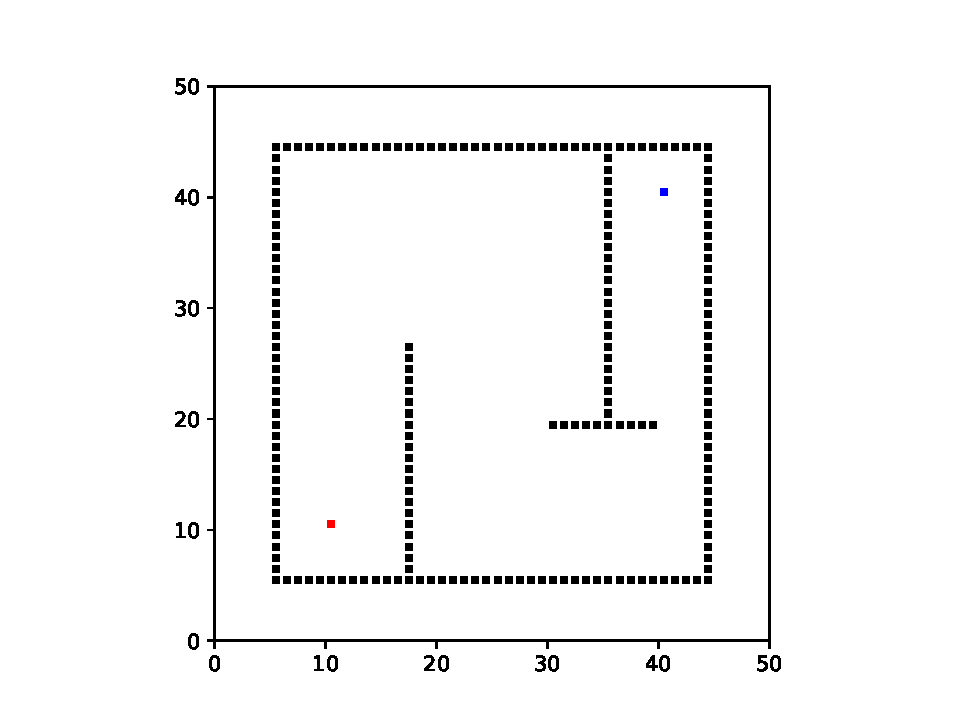
\includegraphics[scale=0.6]{fig/map.pdf}
        \caption{仿真所用空间}
    \end{figure}

    \subsection{深度优先搜索(depth first search)}
    深度优先搜索,下简称深搜,是一种用于遍历搜索图的算法。在路径规划中,深搜往往会不能给出一条最优的路线,但是由于这是一种递归的算法,实现较为方便,在简单的情况下也可以是一种备选的方案。其伪代码如下。

    \begin{algorithm}[H]
        \caption{depth first search}
        \KwIn{a start vertex $s$, an end vertex $t$, the graph $G$}
        \KwOut{a path $p$}
        \For{each $v\in G$}{$father(v)\gets$ -1}
        $father(s)\gets$ 1 \;
        $l \gets$ stack()\;
        $l$.push($s$)\;
        \While{$l$.top()$=t$}{
            $v \gets l$.pop()\;
            \For{each $(u,v)$}{
                \If{$father(u)=-1$}{
                    $father(u)\gets v$\;
                    $l$.push($u$)\;
                }
            } 
        }
        $p \gets $ RECOVER\_PATH($father$)\;
    \end{algorithm}

    \pagebreak
    其仿真效果如下图,其中黑色的点表示障碍,红色为起点,蓝色为终点,绿色点表示搜索过的点,紫色点表示最终所得路径。如图所示,深搜确实得出了一条由起点到终点的路径,但是由于深搜的性质,所得的路径并非是最优的路径。

    \begin{figure}[h]
        \centering
        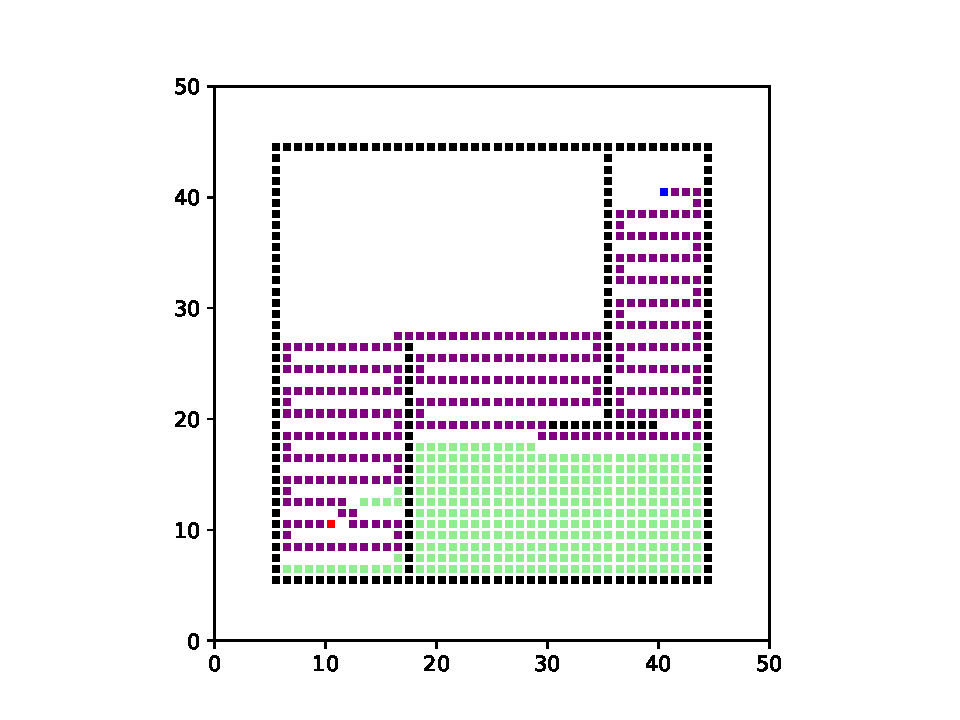
\includegraphics[scale=0.7]{fig/dfs.pdf}
        \caption{深度优先搜索}
    \end{figure}
    \pagebreak
    \subsection{广度优先搜索(breadth first search)}
    如同深度优先搜索,广度优先搜索(以下简称广搜)同样是一种用于遍历图的算法。由于广搜“一层一层”展开的性质,广搜所得的路径为最短路径,事实上无权图中求最短路的算法就是广搜。再加上广搜实现也较为简单方便,在走迷宫等场景中广搜是一种常用的算法。其伪代码如下
    
    \begin{algorithm}[H]
        \caption{breadth first search}
        \KwIn{a start vertex $s$, an end vertex $t$, the graph $G$}
        \KwOut{a path $p$}
        \For{each $v\in G$}{$father(v)\gets$ -1}
        $father(s)\gets$ 1 \;
        $l \gets$ queue()\;
        $l$.push($s$)\;
        \While{$l$.top()$=t$}{
            $v \gets l$.pop()\;
            \For{each $(u,v)$}{
                \If{$father(u)=-1$}{
                    $father(u)\gets v$\;
                    $l$.push($u$)\;
                }
            } 
        }
        $p \gets $ RECOVER\_PATH($father$)\;
    \end{algorithm}

    \pagebreak
    算法运行结果如下。如图可见,广搜算法规划出了一条最短路但是由于其“一层一层”展开的性质,广搜往往需要搜索较多的点才能规划出最优的路径,这就导致了其效率较低的缺点。

    \begin{figure}[h]
        \centering
        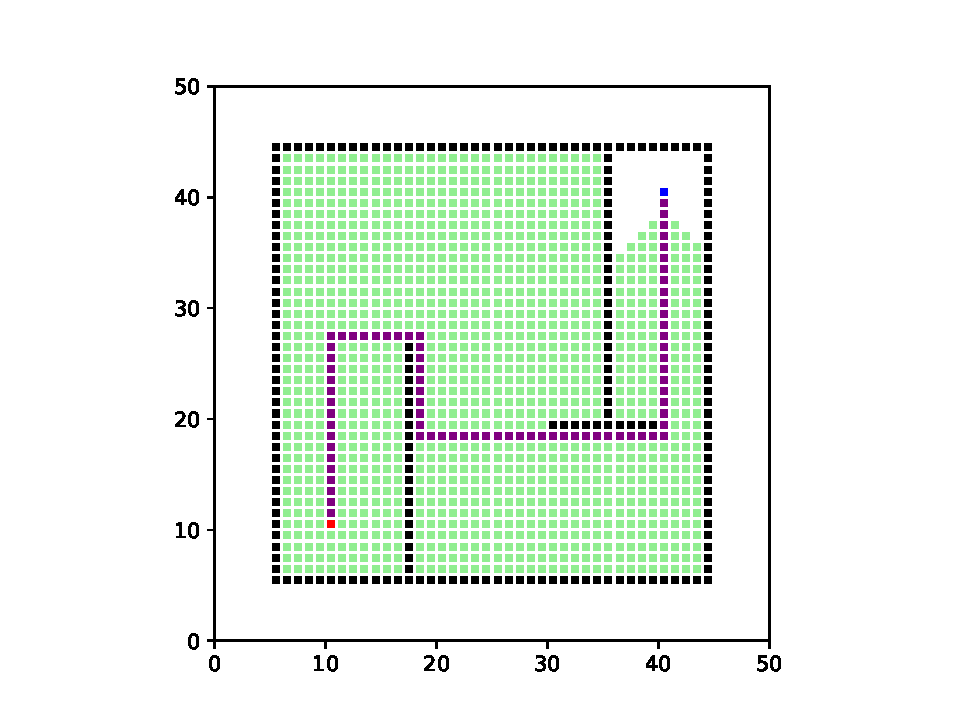
\includegraphics[scale=0.7]{./fig/bfs.pdf}
        \caption{广度优先搜索}
    \end{figure}

    \subsection{A*算法}
    A*算法是一种图的遍历与搜索算法,由于其最优性、高效性,常被用于寻路的算法中。不通用以上两种搜索算法并没有应用终点的信息经行引导加速路径的规划,在A*算法中,我们引入一个启发性函数(heuristic function)$h(n)$,对搜索的过程进行引导,加速搜索的过程。设启发性函数为$h(n)$,起点到当前节点距离为$g(n)$,估计距离$f(n)=g(n)+h(n)$。其中$h(n)$不会高估(overestimate)当前节点到终点距离。则其伪代码如algorithm3。

    \begin{algorithm}[H]
        \caption{A*}
        \KwIn{$s$, $t$, $G$}
        \KwOut{a path $p$}
        \For{each $v\in G$}{
            $g(v)\gets \infty$\;
            $f(v) \gets \infty$\;
        }
        $g(s) \gets h(s)$\;
        $f(s) \gets 0$\;
        $OpenSet \gets \{s\}$\;
        \While(){$OpenSet$ is not empty}{
            $cur \gets \text{arg min}_{\{v \in OpenSet\}} f(v)$\;
            \If(){$cur=t$}{$p \gets $RECOVER\_PATH()\;Return $p$\;}
            $OpenSet \gets OpenSet\backslash \{cur\}$\;
            \For(){each $(u,cur) \in G$}{
                \If(){$f(u)>f(cur)+1$}{
                    $g(u) \gets g(cur)+1$\;
                    $f(u) \gets f(cur)+1$\;
                }
            }
        }
    \end{algorithm}
    
    \pagebreak

    A*算法最优性证明如下:设所得路径为$p$,若$p$不为最优路径,由于算法每次会选取有最小估计距离的节点经行更新,则$p$上一定存在节点$v$使得实际距离$cost(v)>$估计距离$f(v)$,这与条件相悖,故假设不成立。$p$为最优解。

    正是因为算法要求启发性函数$h(n)$不能高估距离,所以八联通和四联通存在着显著区别。在四联通的情况下,曼哈顿距离(实际上也是1-范数)作为$h(n)$,但是如果假设图是八联通的,显然就高估(overestimate)了花费的距离,此时用欧几里得距离,即2-范数才是可用的启发性函数。

    仿真结果如下,可以看到,在启发性函数的引导下,算法遍历较少的点就规划出了一条最优的路径。启发性函数越准确,算法效率就越高。

    \begin{figure}[h]
        \centering
        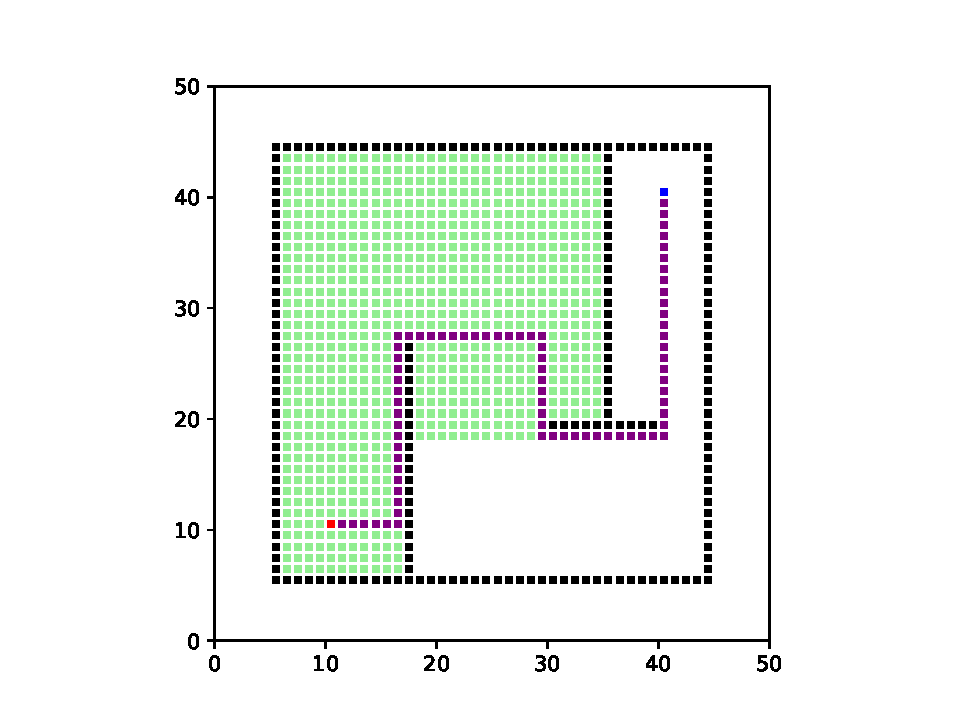
\includegraphics[scale=0.7]{fig/A_star.pdf}
        \caption{A*}
    \end{figure}

    \section{采样算法}
    采样算法不同于搜索算法,具有以下性质。
    \begin{itemize}
        \item 不需要知道空间全貌
        \item 只需要知道当前机器人的碰撞情况
        \item 通过简单的碰撞测试获取信息
    \end{itemize}
    因为以上优点,相比搜索类的算法,这类算法在实际的应用中更加广泛。

    \subsection{RRT算法(rapid-exploring random tree)}
    快速随机搜索树是一种通过构建一颗填满空间的树(space-filling tree)来经行非凸空间搜索的算法。于1998年由 Steven M. LaValle提出。现在与其改进算法(如rrt*、informed-rrt)被广泛应用于路径规划中。

    根据其原论文算法伪代码如algoritm4。

    \begin{algorithm}[H]
        \caption{Generate RRT}
        \KwIn{$x_{init}, K, \varDelta{t}$}
        \KwOut{$\mathcal{T}$}
        $\mathcal{T}$.init($x_{init}$)\;
        \For(){$k=1$ to $K$}{
            $x_{rand} \gets $RANDOM\_STATE()\;
            $x_{near} \gets $NEAREST\_NEIGHBOR($x_{rand},\mathcal{T}$)\;
            $u \gets $SELECT\_INPUT($x_{rand}, x_{near}$)\;
            $x_{new} \gets$NEW\_sTATE($x_{near},u,\varDelta{t}$)\;
            $\mathcal{T}$.add($x_{new}$)\;
            $\mathcal{T}$.add\_edge($x_{new},x_{near}$)\;
        }
    \end{algorithm}

    若根据其原论文在无障碍的空间中经行路径规划效果如图5。可以看到,在这个空间中树的生长较为随意没有很好的指向性,造成采样次数较多,实际运行过程中会导致运行效率较低。
    \begin{figure}[H]
        \centering
        \begin{minipage}[t]{0.45\linewidth}
            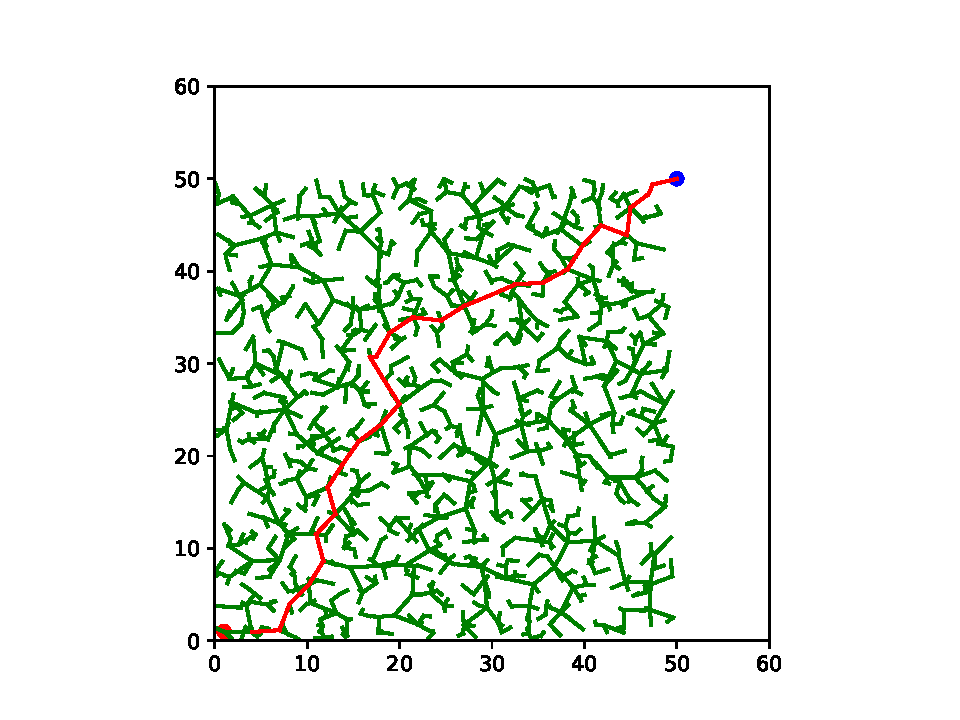
\includegraphics[scale=0.4]{fig/rrt_no_obs.pdf}
            \caption{无引导rrt}
        \end{minipage}
        \begin{minipage}[t]{0.45\linewidth}
            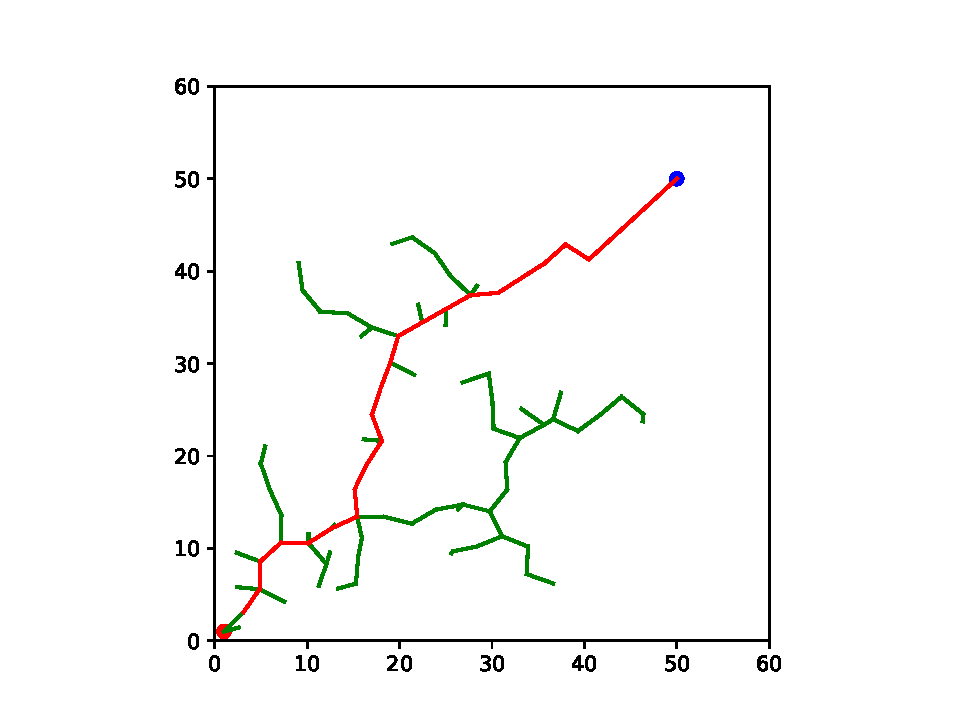
\includegraphics[scale=0.4]{fig/rrt_guide.pdf}
            \caption{有引导rrt}
        \end{minipage}
    \end{figure}

    相应的,我们可以效仿A*算法的思想用终点信息对其经行一定的引导,加快树建立的过程。比如我们可以更加一定的概率将$x_{rand}$改为$x_{goal}$,进行引导,当该概率$p=0.1$时效果如图6。

    加入碰撞检测,并完善生成逻辑即可将rrt用于路径规划算法,其效果如图7、8
    \begin{figure}[htbp]
        \centering
        \subfigure[]{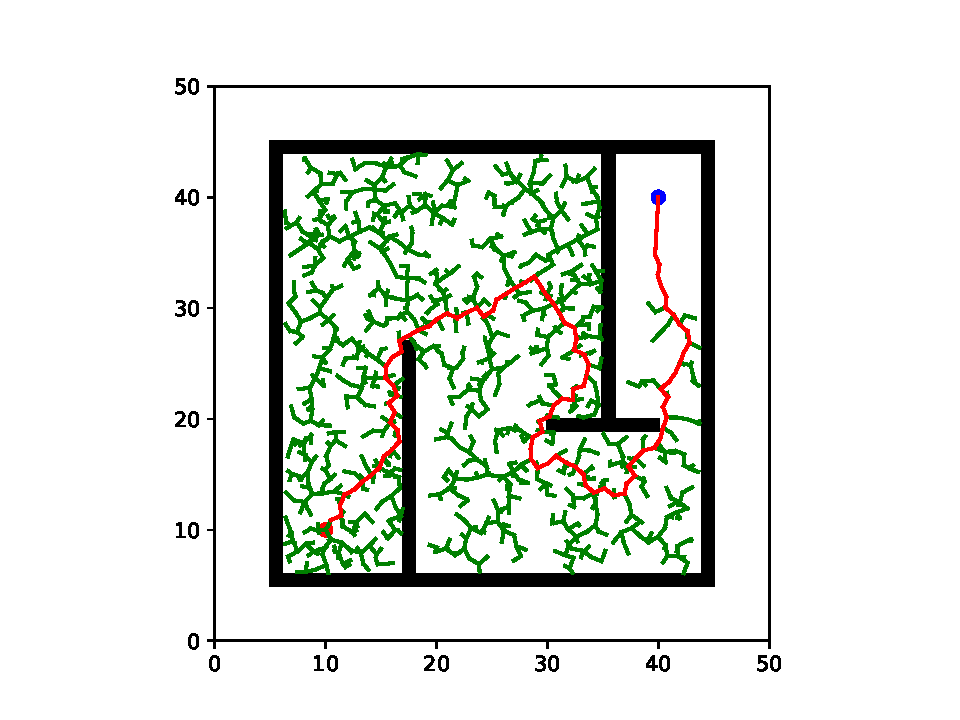
\includegraphics[scale=0.4]{fig/rrt_1.pdf}}
        \subfigure[]{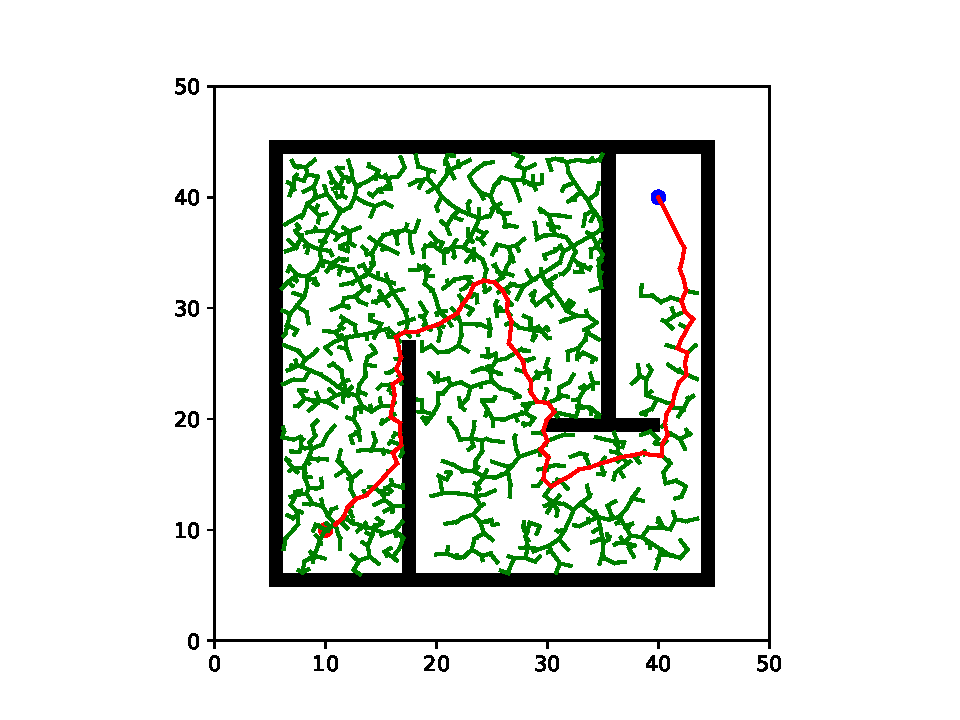
\includegraphics[scale=0.4]{fig/rrt_2.pdf}}
        \caption{ rrt路径规划}
    \end{figure}

    值得一提的是,在实现过程中若有意识地将朝向障碍物的点不作为采样点也可以加快路径搜索的完成,因为这样就相当于引导搜索树不朝向障碍物生长,加速了算法的完成。

    \section{总结}
    本次时间中我主要对一些经典的路径规划算法进行了学习,并结合自身算法基础经行了一定的理解和研究。另外,还使用Python语言经行了对算法的实现与仿真,并完成了结果的可视化。仿真代码完全由我个人完成,并未使用任何开源代码,github仓库会在实践结束后设为public,以供复现检验。

    \section{参考资料}
    \begin{enumerate}
        \item[1] P. E. Hart, N. J. Nilsson and B. Raphael, "A Formal Basis for the Heuristic Determination of Minimum Cost Paths," in IEEE Transactions on Systems Science and Cybernetics, vol. 4, no. 2, pp. 100-107, July 1968, doi: 10.1109/TSSC.1968.300136.
        \item[2] LaValle, Steven M. (October 1998). "Rapidly-exploring random trees: A new tool for path planning" (PDF). Technical Report. Computer Science Department, Iowa State University (TR 98–11).
        \item[3] Delling, D.; Sanders, P.; Schultes, D.; Wagner, D. (2009). "Engineering Route Planning Algorithms"
        \item[4] 维基百科(wikipedia)  
        \item[5] github开源项目https://github.com/zhm-real/PathPlanning 
    \end{enumerate}
\end{document}
